\documentclass[pdftex,a4paper,titlepage,11pt,openright]{article}
\usepackage[T1]{fontenc}
\usepackage[utf8]{inputenc}
\usepackage[english,francais]{babel}
\usepackage{listings}
\usepackage{setspace}

\usepackage{avant}
\usepackage{fancyvrb}
\usepackage{fancyhdr}
\pagestyle{fancy}
\fancyhf{}
\fancyhead[LE,RO]{\itshape\thepage}
% \fancyhead[LO]{\itshape\rightmark}
% \fancyhead[RE]{\itshape\leftmark}
\renewcommand{\headrulewidth}{0.5pt}
\usepackage[top=2.5cm, bottom=2.5cm, left=3.0cm, right=3.0cm, a4paper]{geometry}
% \addtolength{\headheight}{0.5pt}
% \renewcommand\footrulewidth{0pt}
\fancypagestyle{plain}{
    \fancyhead{}
    \renewcommand{\headrulewidth}{0pt}}
\usepackage{textcomp}
\usepackage{relsize}
\usepackage{amssymb}
\usepackage[colorlinks=true,linkcolor=black,citecolor=black,urlcolor=black,filecolor=black]{hyperref}
\usepackage{framed}
\usepackage[pdftex]{graphicx}
\usepackage{makeidx}
% \addtolength{\textwidth}{1cm}
% \setlength{\textheight}{24cm} 	% Hauteur de la zone de texte


% nouvelle commande pour un joli nom
\newcommand{\nom}[1]{\textsc{#1}}

% commande pour une zolie ligne
\newcommand{\ligne}[1][1pt]{
  \par\noindent
  \rule[.5ex]{\linewidth}{#1}\par}

% nettoyer une page blanche avant une page de chapitre en mode openright
\newcommand{\clearemptydoublepage}{
	\newpage{\pagestyle{empty}\cleardoublepage}}


\makeindex

\begin{document}

% augmenter l'espacement entre plusieurs paragraphes plutôt que de passer des lignes quand il faut pas
\setlength{\parskip}{2.4ex}

\title{
\ligne{\Large}
\textbf{Audit Security}\\
\textbf{Project de deuxième année}\\
\Large Remplacement et généralisation des plugins contextd
\ligne{\Large}
}
\author{\nom{Dimitri Gressin} \& \nom{Timothée Ravier}\\\\\nom{Pilote : Jérémy Briffaut}}
\date{xx xxx 2011} %TODO

% titre
\maketitle

% page blanche
\clearemptydoublepage

% table des matières
\setcounter{secnumdepth}{2}
\setcounter{tocdepth}{2}
\addtocontents{toc}{\protect\thispagestyle{empty}}
\tableofcontents
\addtocounter{page}{-1}

\newpage

\section*{Introduction} \addcontentsline{toc}{section}{Introduction}
Ce rapport présente le travail et les résultats obtenus à la fin du premier semestre, dans le cadre de notre projet d'application de deuxième année.
%TODO

~

Le but de ce projet est de généraliser la communication entre les différentes applications exécutées sur PIGA-OS et le daemon contextd. 
Ce daemon recueil auprès de celles-ci les différentes opérations qu'elles effectuent (lecture/écriture de fichiers, création de socket, etc.) pour en déduire un contexte.
Jusqu'à présent, la communication entre les applications et contextd s'effectuait via un pluging propre à chaque application. Le but de ce projet est donc de s'affranchir de l'utilisation relativement contraignante de ces plugings (il fallait en developper un pour chaque application, et pour chaque version de celles-ci). 

L'idée retenue est de déplacer les actions effectuées par le pluging au niveau du noyau par l'intermédiaire des appels systèmes.


\newpage

\section{Objectifs}

Pour pouvoir se séparer des plugins/modifications par applications, il est nécessaire de communiquer à contextd certaines informations sur le comportement des programmes. Il faut notamment obtenir :
\begin{itemize}
	\item la liste des fichiers créés, ouverts, modifiés par l'ensemble des processus, et les contextes SELinux associés, si le module SELinux est activé.
	\item la liste des connexions ouvertes par le systeme, et plus particulièrement les adresses IP de destination, et donc finalement le nom de domaine de destination.\\
\end{itemize}

De plus, il faut que le programme puisse attendre la réponse de contextd avant de poursuivre son exécution.

\section{Systemtap}

\subsection{Principe de fonctionnement}

Nous avons ainsi commencer par utiliser Systemtap, un outil d'analyse du noyau grâce à des scripts qui ne nécessite pas de modifier le code du noyau. Systemtap utilise les KProbes, et les Kretprobes\cite{IBMRBST} pour intervenir à différents endroits dans le déroulement des fonctions du noyau pour permettre à l'utilisateur de lire certaines variables ou de logger certains appel système. Le principe de fonctionnement de Systemtap est résumé sur le schéma ci-dessous.
\begin{figure}[hb]
	\centering
	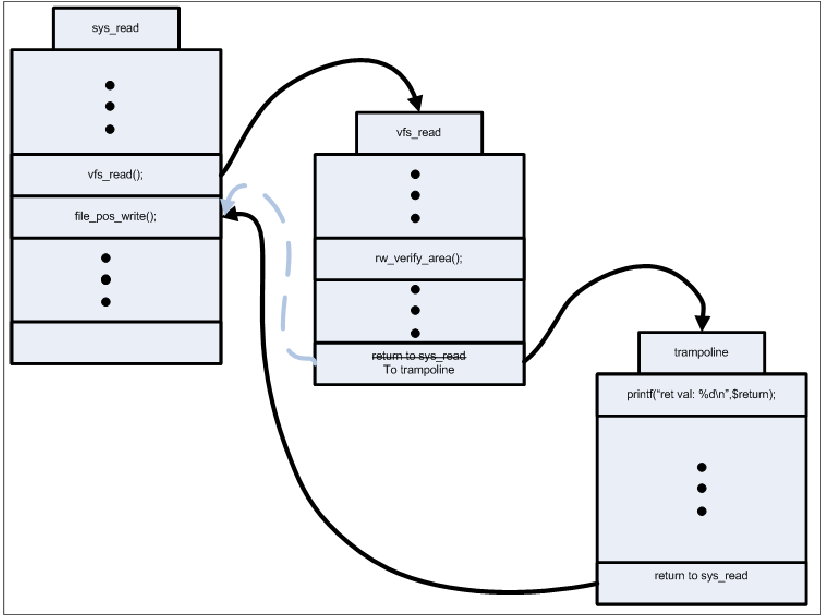
\includegraphics[scale=0.4]{kretprob.png}
	\caption{Fonctionnement tel que décrit dans la référence IBM sur Systemtap \cite{IBMRBST}}
\end{figure}

\subsection{Résultats obtenus}

Après s'être familiarisé avec le fonctionnement de Systemtap, nous nous sommes aperçu que les scripts utilisés pour récupérer les informations issues des appels système sont exécutés une fois l'appel système effectué. Il ne nous est pas possible, d'après nos recherches, de faire en sorte que les scripts puissent bloquer les appels systèmes avant de les effectués.

De ce fait, l'utilisation de Systemtap ne permet pas de répondre à nos besoins.

Il faut ajouter à cela que les informations recueillies à partir de Systemtap ne sont pas exploitables pour certaines d'entre-elles. Par exemple, lorsqu'un fichier est accédé (lu ou écrit), seul le numéro d'inode nous était retourné. Il ne nous était impossible alors de récupérer le chemin complet du fichier.

Il fallait donc changer de stratégie. C'est pourquoi, nous avons, avec l'accord du responsable du projet, Jérémy Briffaut, de nous orienter vers l'utilisation d'un module LSM.

%\includegraphics[scale=0.4]{stap_internals.png} TODO


\newpage


\section{Linux Security Modules}



\subsection{Principe de fonctionnement}

Les modules LSM sont au noyau ce que iptables est au réseau. 

Le principe de fonctionnement est simple. Le module LSM est chargé dans le noyau Linux au démarrage. Une fois chargé, il se place entre l'appel système et l'exécution de celui-ci par l'intermédiaire de hooks. A chaque appel système est associé un hook que l'on peut considéré comme une fonction. Dès qu'un appel système est demandé, le hook est exécuté. Par défaut, il renvoie 0 pour autoriser l'exécution de l'appel système. Toute valeur différente de 0 bloque l'appel système (et possiblement le programme à l'origine de l'appel).



\begin{figure}[hb]
	\centering
	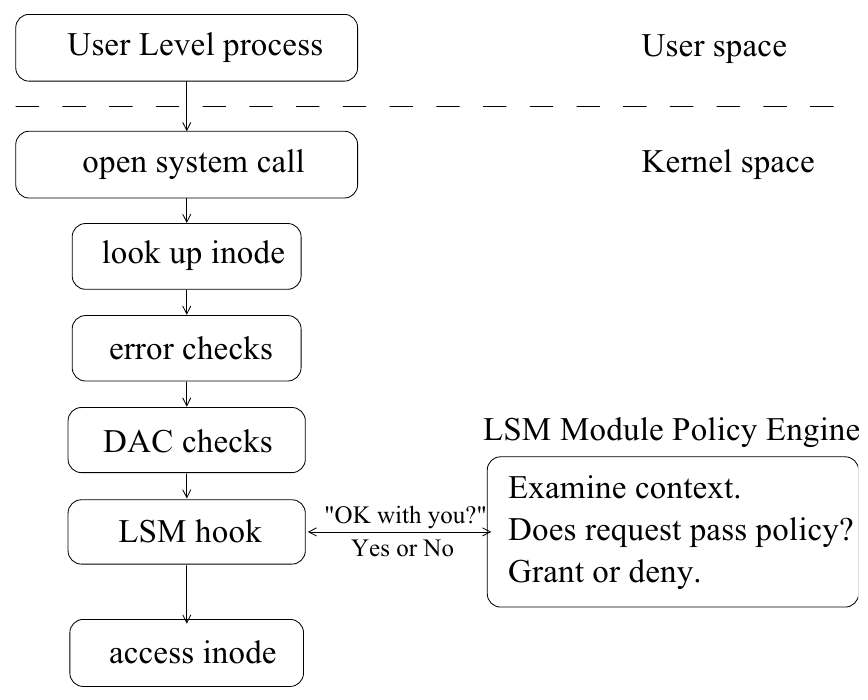
\includegraphics[scale=0.45]{lsm1.png}
	\caption{LSM Hook Architecture \cite{LSMINTRO}}
\end{figure}

\begin{figure}[hb]
	\centering
	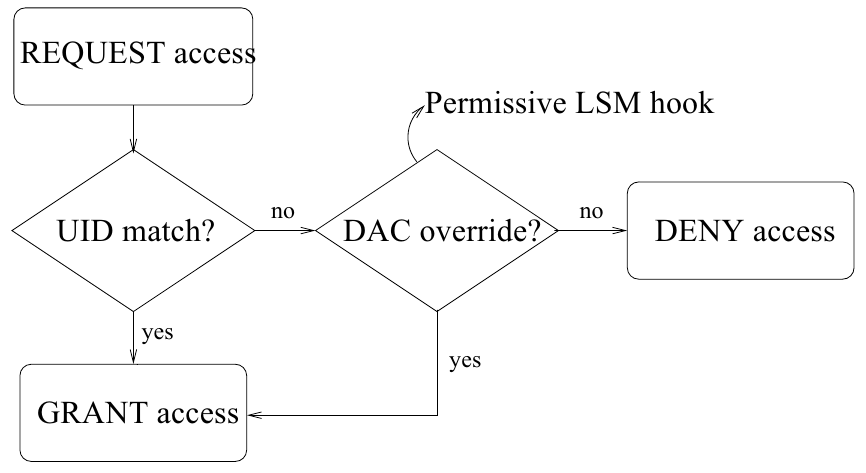
\includegraphics[scale=0.45]{lsm2.png}
	\caption{Permissive LSM hook. This hook allows the security policy to override a DAC restriction \cite{LSMINTRO}}
\end{figure}

L'avantage de ces hooks est qu'ils offrent une très grande liberté. Cependant, il n'est possible pour le moment que de chargé dans le noyau qu'un seul et unique module LSM. Or, PIGA-OS utilise déjà un module LSM : SELinux.

Pour les besoins du développement, nous avons dû donc désactiver SELinux.

\newpage

\subsection{Ce qui a été réalisé}

Nous avons donc développé un module LSM qui "hook" tous les appels systèmes. Par défaut, ces hooks sont "transparents" à l'excéption du hook "file permission" sur lequel nous travaillons. Par la suite, il faudra convenir des appels systèmes surlesquels il est intéressant d'intervenir.

Nous avons ajouté la possibilité d'activer ou non ce module lors de la compilation du noyau en ajoutant un choix dans menuconfig.

Ensuite, nous avons commencer à chercher les différentes informations nécessaires à contextd pour son fonctionnement concernant le hook "file permission" à savoir :
	\begin{itemize}
		\item[-] le PID
		\item[-] l'execname
		\item[-] le chemin complet du fichier accédé (lecture/écriture/exécution)
		\item[-] ...
	\end{itemize}

Nous avons également remarqué que le hook "socket bind" permet de récupérer des informations avant qu'une socket soit créée comme :
	\begin{itemize}
		\item[-] le PID
		\item[-] l'execname
		\item[-] la structure de la socket
		\item[-] L'adresse de connexion
		\item[-] ...
	\end{itemize}

La principal difficulté de cette étape est de localisé dans quels fichiers ses informations sont localisés dans l'ensemble du code source du noyau Linux.



\newpage

\clearemptydoublepage

\section*{Conclusion} \addcontentsline{toc}{section}{Conclusion}

%Ce projet aura été pour nous l'occasion d'apprendre un langage de programmation orienté objets, qui nous a permis de gagner en efficacité lors de la phase de développement. En revanche, le fait que nous découvrions le C++ a limité nos possibilités d'optimisations. Le temps de traitement d'un graphe contenant une grande quantité de noeud étant élevé, il paraît nécessaire de paralléliser les algorithmes que nous avons appliqués, pour tirer pleinement partie des machines multi-coeurs ou multi-processeurs, par exemple en utilisant les Intel Threading Building Blocks \cite{IBMRBST}.

%De plus, bien que vérifiée, notre implémentation de l'algorithme de décomposition modulaire peut contenir des bugs. Il faut donc prévoir un outils permettant la vérification des résultats obtenus par cette méthode avec ceux obtenus par le parcours simple de graphes. Il sera donc toujours nécessaire de produire l'intégralité des chemins entre deux noeuds à partir du graphe d'origine pour s'assurer que les graphes réduits sont bien justes.

%Il faut noter, au vu des résultats, que la décomposition modulaire de graphes permettra fort probablement non seulement d'accélerer le parcours de graphes une fois l'intégralité des chemins générés mais aussi de réduire la taille finale de l'ensemble formé par tous les chemins.

%Enfin, notre programme se limite à la décomposition de graphes orientés. Les algorithmes diffèrent de ceux applicables aux graphes non-orientés et leur mise en oeuvre nécessiterai la réécriture d'une grande partie du code pour assurer la rapidité et l'efficacité de notre implémentation.


\newpage
\addcontentsline{toc}{section}{Annexes}
\addcontentsline{toc}{subsection}{Remarques}
\addcontentsline{toc}{subsection}{Liens et références}
\subsection*{Remarques}

%Un fichier de configuration est présent avec les sources du kernel 2.6.32-hardened. Il correspond aux options nécessaire à la compilation dans une machine virtuelle Virtualbox. L'option autorisant nos modifications y est aussi activée. Elle est situé dans Security -> SELinux userspace audit.

\subsection*{Liens et références}
\begin{thebibliography}{40}
\bibitem{IBMRBST} \textit{IBM Redbooks : SystemTap: Instrumenting the Linux Kernel for Analyzing Performance and Functional Problems}, \url{http://www.redbooks.ibm.com/abstracts/redp4469.html}

\bibitem{LSMINTRO} \textit{Linux Security Modules : General Security Support for the Linux Kernel}, \url{http://citeseerx.ist.psu.edu/viewdoc/download?doi=10.1.1.84.6867&rep=rep1&type=pdf}

\bibitem{SOURCE} Code source (kernel 2.6.32 hardened r9 et scripts systemtap) disponible sur le serveur de projet STI (le projet s'appelle pour l'instant ``Projet LSM''), \url{http://projetsti.ensi-bourges.fr/projects/promo2012-systemtap}.

\bibitem{LKDSE} \textit{Linux Kernel Development, Second Edition}, Robert Love, Novell Press
\end{thebibliography}

%\printindex

\end{document}
